\documentclass[twoside]{book}

% Packages required by doxygen
\usepackage{calc}
\usepackage{doxygen}
\usepackage{graphicx}
\usepackage[utf8]{inputenc}
\usepackage{makeidx}
\usepackage{multicol}
\usepackage{multirow}
\usepackage{textcomp}
\usepackage[table]{xcolor}

% Font selection
\usepackage[T1]{fontenc}
\usepackage{mathptmx}
\usepackage[scaled=.90]{helvet}
\usepackage{courier}
\usepackage{amssymb}
\usepackage{sectsty}
\renewcommand{\familydefault}{\sfdefault}
\allsectionsfont{%
  \fontseries{bc}\selectfont%
  \color{darkgray}%
}
\renewcommand{\DoxyLabelFont}{%
  \fontseries{bc}\selectfont%
  \color{darkgray}%
}

% Page & text layout
\usepackage{geometry}
\geometry{%
  a4paper,%
  top=2.5cm,%
  bottom=2.5cm,%
  left=2.5cm,%
  right=2.5cm%
}
\tolerance=750
\hfuzz=15pt
\hbadness=750
\setlength{\emergencystretch}{15pt}
\setlength{\parindent}{0cm}
\setlength{\parskip}{0.2cm}
\makeatletter
\renewcommand{\paragraph}{%
  \@startsection{paragraph}{4}{0ex}{-1.0ex}{1.0ex}{%
    \normalfont\normalsize\bfseries\SS@parafont%
  }%
}
\renewcommand{\subparagraph}{%
  \@startsection{subparagraph}{5}{0ex}{-1.0ex}{1.0ex}{%
    \normalfont\normalsize\bfseries\SS@subparafont%
  }%
}
\makeatother

% Headers & footers
\usepackage{fancyhdr}
\pagestyle{fancyplain}
\fancyhead[LE]{\fancyplain{}{\bfseries\thepage}}
\fancyhead[CE]{\fancyplain{}{}}
\fancyhead[RE]{\fancyplain{}{\bfseries\leftmark}}
\fancyhead[LO]{\fancyplain{}{\bfseries\rightmark}}
\fancyhead[CO]{\fancyplain{}{}}
\fancyhead[RO]{\fancyplain{}{\bfseries\thepage}}
\fancyfoot[LE]{\fancyplain{}{}}
\fancyfoot[CE]{\fancyplain{}{}}
\fancyfoot[RE]{\fancyplain{}{\bfseries\scriptsize Generated on Sat Aug 19 2017 05\-:25\-:32 for G\-H\-O\-S\-T by Doxygen }}
\fancyfoot[LO]{\fancyplain{}{\bfseries\scriptsize Generated on Sat Aug 19 2017 05\-:25\-:32 for G\-H\-O\-S\-T by Doxygen }}
\fancyfoot[CO]{\fancyplain{}{}}
\fancyfoot[RO]{\fancyplain{}{}}
\renewcommand{\footrulewidth}{0.4pt}
\renewcommand{\chaptermark}[1]{%
  \markboth{#1}{}%
}
\renewcommand{\sectionmark}[1]{%
  \markright{\thesection\ #1}%
}

% Indices & bibliography
\usepackage{natbib}
\usepackage[titles]{tocloft}
\setcounter{tocdepth}{3}
\setcounter{secnumdepth}{5}
\makeindex

% Hyperlinks (required, but should be loaded last)
\usepackage{ifpdf}
\ifpdf
  \usepackage[pdftex,pagebackref=true]{hyperref}
\else
  \usepackage[ps2pdf,pagebackref=true]{hyperref}
\fi
\hypersetup{%
  colorlinks=true,%
  linkcolor=blue,%
  citecolor=blue,%
  unicode%
}

% Custom commands
\newcommand{\clearemptydoublepage}{%
  \newpage{\pagestyle{empty}\cleardoublepage}%
}


%===== C O N T E N T S =====

\begin{document}

% Titlepage & ToC
\hypersetup{pageanchor=false}
\pagenumbering{roman}
\begin{titlepage}
\vspace*{7cm}
\begin{center}%
{\Large G\-H\-O\-S\-T }\\
\vspace*{1cm}
{\large Generated by Doxygen 1.8.6}\\
\vspace*{0.5cm}
{\small Sat Aug 19 2017 05:25:32}\\
\end{center}
\end{titlepage}
\clearemptydoublepage
\tableofcontents
\clearemptydoublepage
\pagenumbering{arabic}
\hypersetup{pageanchor=true}

%--- Begin generated contents ---
\chapter{G\-H\-O\-S\-T}
\label{index}\hypertarget{index}{}G\-H\-O\-S\-T documentation \begin{DoxyAuthor}{Author}
Florian Richoux
\end{DoxyAuthor}
\section*{Introduction }

G\-H\-O\-S\-T (General meta-\/\-Heuristic Optimization Solving Tool) is a C++11 library designed for Star\-Craft\-: Brood war. G\-H\-O\-S\-T implements a meta-\/heuristic solver aiming to solve any kind of combinatorial and optimization R\-T\-S-\/related problems represented by a C\-S\-P. It is an generalization of the Wall-\/in project (see \href{https://github.com/richoux/Wall-in}{\tt github.\-com/richoux/\-Wall-\/in}).

The source code is available at \href{https://github.com/richoux/GHOST}{\tt github.\-com/richoux/\-G\-H\-O\-S\-T}, and the documentation pages at \href{http://richoux.github.io/GHOST}{\tt richoux.\-github.\-io/\-G\-H\-O\-S\-T}. G\-H\-O\-S\-T is under the terms of the G\-N\-U G\-P\-L v3 licence.

\subsection*{Scientific papers\-: }


\begin{DoxyItemize}
\item Florian Richoux, Jean-\/\-François Baffier and Alberto Uriarte, G\-H\-O\-S\-T\-: A Combinatorial Optimization Solver for R\-T\-S-\/related Problems (to appear).
\item Florian Richoux, Alberto Uriarte and Santiago Ontañón, Walling in Strategy Games via Constraint Optimization (to appear in A\-I\-I\-D\-E 2014 proceedings).
\item Santiago Ontañón, Gabriel Synnaeve, Alberto Uriarte, Florian Richoux, David Churchill and Mike Preuss, \href{http://pagesperso.lina.univ-nantes.fr/~richoux-f/publications/tciaig13.pdf}{\tt A Survey of Real-\/\-Time Strategy Game A\-I Research and Competition in Star\-Craft}, Transactions on Computational Intelligence and A\-I in Games, I\-E\-E\-E, 2013.
\end{DoxyItemize}

\section*{A short C\-S\-P/\-C\-O\-P tutorial }

T\-O\-D\-O

\section*{How to use G\-H\-O\-S\-T? }

T\-O\-D\-O

\section*{How to define and solve my own C\-S\-P problem with G\-H\-O\-S\-T? }

T\-O\-D\-O 
\chapter{File Index}
\section{File List}
Here is a list of all files with brief descriptions\-:\begin{DoxyCompactList}
\item\contentsline{section}{include/\hyperlink{solver_8hpp}{solver.\-hpp} }{\pageref{solver_8hpp}}{}
\item\contentsline{section}{include/constraints/\hyperlink{constraint_8hpp}{constraint.\-hpp} }{\pageref{constraint_8hpp}}{}
\item\contentsline{section}{include/constraints/\hyperlink{wallinConstraint_8hpp}{wallin\-Constraint.\-hpp} }{\pageref{wallinConstraint_8hpp}}{}
\item\contentsline{section}{include/domains/\hyperlink{domain_8hpp}{domain.\-hpp} }{\pageref{domain_8hpp}}{}
\item\contentsline{section}{include/domains/\hyperlink{wallinDomain_8hpp}{wallin\-Domain.\-hpp} }{\pageref{wallinDomain_8hpp}}{}
\item\contentsline{section}{include/misc/\hyperlink{constants_8hpp}{constants.\-hpp} }{\pageref{constants_8hpp}}{}
\item\contentsline{section}{include/misc/\hyperlink{races_8hpp}{races.\-hpp} }{\pageref{races_8hpp}}{}
\item\contentsline{section}{include/misc/\hyperlink{random_8hpp}{random.\-hpp} }{\pageref{random_8hpp}}{}
\item\contentsline{section}{include/misc/\hyperlink{wallinProtoss_8hpp}{wallin\-Protoss.\-hpp} }{\pageref{wallinProtoss_8hpp}}{}
\item\contentsline{section}{include/misc/\hyperlink{wallinTerran_8hpp}{wallin\-Terran.\-hpp} }{\pageref{wallinTerran_8hpp}}{}
\item\contentsline{section}{include/objectives/\hyperlink{objective_8hpp}{objective.\-hpp} }{\pageref{objective_8hpp}}{}
\item\contentsline{section}{include/objectives/\hyperlink{wallinObjective_8hpp}{wallin\-Objective.\-hpp} }{\pageref{wallinObjective_8hpp}}{}
\item\contentsline{section}{include/variables/\hyperlink{building_8hpp}{building.\-hpp} }{\pageref{building_8hpp}}{}
\item\contentsline{section}{include/variables/\hyperlink{variable_8hpp}{variable.\-hpp} }{\pageref{variable_8hpp}}{}
\item\contentsline{section}{src/\hyperlink{main_8cpp}{main.\-cpp} }{\pageref{main_8cpp}}{}
\item\contentsline{section}{src/constraints/\hyperlink{wallinConstraint_8cpp}{wallin\-Constraint.\-cpp} }{\pageref{wallinConstraint_8cpp}}{}
\item\contentsline{section}{src/domains/\hyperlink{wallinDomain_8cpp}{wallin\-Domain.\-cpp} }{\pageref{wallinDomain_8cpp}}{}
\item\contentsline{section}{src/objectives/\hyperlink{wallinObjective_8cpp}{wallin\-Objective.\-cpp} }{\pageref{wallinObjective_8cpp}}{}
\item\contentsline{section}{src/variables/\hyperlink{building_8cpp}{building.\-cpp} }{\pageref{building_8cpp}}{}
\item\contentsline{section}{src/variables/\hyperlink{variable_8cpp}{variable.\-cpp} }{\pageref{variable_8cpp}}{}
\end{DoxyCompactList}

\chapter{File Documentation}
\hypertarget{mainpage_8dox}{\section{doc/mainpage.dox File Reference}
\label{mainpage_8dox}\index{doc/mainpage.\-dox@{doc/mainpage.\-dox}}
}

\hypertarget{variable_8cpp}{\section{src/variable.cpp File Reference}
\label{variable_8cpp}\index{src/variable.\-cpp@{src/variable.\-cpp}}
}
{\ttfamily \#include $<$algorithm$>$}\\*
{\ttfamily \#include $<$typeinfo$>$}\\*
{\ttfamily \#include \char`\"{}variable.\-hpp\char`\"{}}\\*
Include dependency graph for variable.\-cpp\-:
\nopagebreak
\begin{figure}[H]
\begin{center}
\leavevmode
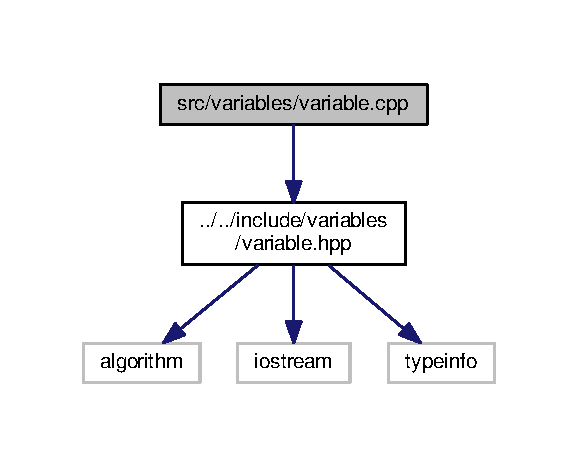
\includegraphics[width=292pt]{variable_8cpp__incl}
\end{center}
\end{figure}

%--- End generated contents ---

% Index
\newpage
\phantomsection
\addcontentsline{toc}{chapter}{Index}
\printindex

\end{document}
